\section{Evaluace modelů}

Jedna z~klíčových aspektů strojového učení je, aby natrénovaný model byl schopný generalizace -- fungovat dobře na nových vstupech.

Při trénování můžeme natrénovat celou řadu modelů (např. ze stejné rodiny ale s~různými sadami hyperparametrů). Pro to, abychom mohli modely porovnat, potřebujeme mít nějakou kvantitativní míru výkonnosti -- metriku. To jakou zvolíme často záleží na charakteru problému. Někdy chceme minimalizovat drobné chyby, někdy celkovou chybovost, apod.

\subsection{Ztrátová funkce}

Uvažujme model natrénovaný na vstupu $\X$ s~vysvětlovanou proměnnou $Y$. Takový model zpravidla není dokonalý a pro $\X$ predikuje nějaké $\hat{Y} \equiv \hat{Y}(\X)$. Funkci $L$, měřící chybu této predikce, nazýváme ztrátovou funkcí (loss function).

\paragraph{Regrese} V~případě regrese je typická kvadratická ztrátová funkce (squared error): \[L(Y, \hat{Y}) = (Y - \hat{Y})^2, \] případně $L_1$  ztrátová funkce měřící absolutní chybu (absolute error): \[L(Y, \hat{Y}) = |Y - \hat{Y}|.\]

\paragraph{Klasifikace} U~binární klasifikace se často odhaduje pravděpodobnost \[\hat{p} = \hat{P}(Y=1 \mid \X = \x),\] pro kterou se nabízí následující ztrátová funkce (binary cross-entropy loss function) \[L(Y, \hat{Y}) = -Y\log\hat{p} - (1-Y)\log(1-\hat{p})\]

\subsubsection{Trénovací chyba}

Při trénování se snažíme minimalizovat průměrnou hodnotu ztrátové chyby přes všechny prvky v~trénovací množině (trénovací chybu, test error): \[\overline{\err}_\train = \mathcal{L} = \frac{1}{N} \sum_{i=1}^{N} L(Y_i, \hat{Y}(\x_i))\]

V~případě regrese se tedy bude jednat například o:
\[
    \MSE_\train = \frac{1}{N} \sum_{i=1}^{N} (Y - \hat{Y})^2
    \quad \text{nebo} \quad
    \MAE_\train = \frac{1}{N} \sum_{i=1}^{N} |Y - \hat{Y}|
\]

A~u~binární klasifikaci o:
\[
    \mathcal{L} = \frac{1}{N} \sum_{i=1}^{N}
    \left[
        - Y_i\log\hat{p}(\x_i) - (1-Y_i)\log(1-\hat{p}(\x_i))]
    \right]
\]

Řešení minimalizující trénovací chybu (test error) lze u~některých modelů spočíst explicitně (closed-form solution), např. u~lin. regrese. Pro většinu modelů to nelze a musíme jej počítat numericky iterativními metodami (např. gradientním sestupem).

\subsubsection{Testovací chyba}

Testovací chyba (test error) je střední chyba na novém vstupu $\X$ při dané trénovací množině $\D$:
\[
    \Err_\D = \E (L(Y, \hat{Y}(\X)) \mid \D)
\]
kterou můžeme odhadnout
\[
    \overline{\err}_\test = \frac{1}{N_\test} \sum_{i=1}^{N_\test} (L(Y_i, \hat{Y}(\x_i))
\]

Nejobecnější mírou schopnosti modelu generalizovat je očekávaná testovací chyba (expected test error), která je střední hodnotou testovací chyby pro náhodný výběr trénovací množiny $\D$:
\[
    \Err = \E (\Err_\D) = \E (L(Y, \hat{Y}(\X)))
\]
Jedná se tedy odhad $\Err_\D$ s~neznámým $\D$.

\subsection{Evaluační scénáře}

Z~pohledu evaluace máme dva úkoly:
\begin{itemize}
    \item Výběr modelu - odhadnout chybu různých modelů za účelem výběru nejlepšího.
    \item Ohodnocení modelu - odhadnout testovací chybu finálního modelu.
\end{itemize}

\subsubsection{Hold-out}

Pokud máme dostatek dat, dělíme data na část
\begin{itemize}
    \item Trénovací - k~natrénování konkrétních modelů.
    \item Validační - k~výběru nejlepší sady hyperparametrů.
    \item Testovací - k~odhadu testovací chyby, kterou očekáváme na nových datech.
\end{itemize}
Pro získání neoptimistického odhadu výkonnosti modelu, musí být testovací část skutečně nový vstup, který nijak neovlivnil parametry ani volbu modelu.

\subsubsection{k-fold cross-validation}

Pokud nemáme dostatek dat, je často nerozumné je dělit na trénovací, validační a testovací. Vedlo by to na nedostatek dat pro správně natrénovaní, dobrou volbu správného modelu a spolehlivého odhadu testovací chyby.

S~křížovou validací se obejdeme bez validační množiny.
\begin{algorithm}[H]
    \renewcommand{\thealgorithm}{}
    \caption{Cross-validation}
    \begin{algorithmic}[1]
        \Require $2 \le k \le N$
        \item Trénovací data $\D$ rozděl na $k$ podobně velkých podmnožin $\D_1, \ldots, \D_k$.
        \item Pro $j = 1, \ldots, k$ natrénuj model s~danými hyperparametry na $\D \setminus \D_j$.
        \item Na $\D_j$ odhadni chybu modelu $e_j$.
        \item \Return cross-validation error
        \[\hat{e} = \frac{1}{k} \sum_{i=1}^{k} e_i\]
    \end{algorithmic}
\end{algorithm}

Takto odhadneme cross-validační chybu pro všechny uvažované sady hyperparametrů a zvolíme model s~nejnižší takovou chybou. Zvolený model s~nejlepšími hyperparametry natrénujeme na celé množině $\D$.

Volba $k$ je kvůli výpočetním nárokům obvykle malá (5, 10). Pro velmi malé datasety může však být únosná i volba $k=N$ (leave-one-out cross-validation).

\paragraph{Cross-validation error} Cross-validation error je odhad očekávané testovací chyby $\Err$ a ne testovací chyby $\Err_\D$.

Při skutečně malém datasetu je možné zvolit dvoustupňovou křížovou validaci, která si neodkládá testovací sadu, ale zanořuje se s~křížovou validací o~jednu stupeň níž, přičemž vnitřní cross-validační chyba se používá pro výběr modelu a vnější pro odhad očekávané chyby.

Vnější cross-validation chyba je pouze jedna (``společná'') a odpovídá očekávané testovací chybě celé procedury pro výběr nejlepšího
modelu, ale nejlepší model teprve musíme získat (natrénování zvoleného modelu na celé množině $\D$).

\paragraph{Finální model} Ve všech metodách lze po výsledném odhadu testovací chyby přetrénovat nejlepší model na celém datasetu a pro odhad výkonnosti použít testovací chybu, resp. očekávanou testovací chybu, z~předchozího kroku. U~hold-out lze před evaluací na trénovacích datech ještě přetrénovat model na (trénovací + validační) množině.

\subsection{Evaluace regrese}

Nejčastější volba ztrátové funkce u~regresních úloh je MSE (mean squared error) nebo MAE (mean absolute error):
\[
    \MSE = \frac{1}{N} \sum_{i=1}^{N} (Y_i - \hat{Y}_i)^2
    \qquad
    \MAE = \frac{1}{N} \sum_{i=1}^{N} |Y_i - \hat{Y}_i|
\]
Zatímco MSE je citlivější na velká residua, MAE se spíše soustředí na celkovou chybu a odlehlým hodnotám se chová ``spravedlivě''. Jednotky MSE jsou v~kvadrátech, proto se také často udává přeškálované RMSE, které má interpretovatelné jednotky vysvětlované proměnné:
\[
    \RMSE = \sqrt{\frac{1}{N} \sum_{i=1}^{N} (Y_i - \hat{Y}_i)^2}
\]

Pro nezáporné hodnoty lze použít ztrátovou funkcí RMSLE, které se soustředí na relativní míru odchylek:
\[
    \RMSLE = \sqrt{\frac{1}{N} \sum_{i=1}^{N} (\log Y_i - \log \hat{Y}_i)^2}
    = \sqrt{\frac{1}{N} \sum_{i=1}^{N} \log^2 \frac{Y_i}{\hat{Y}_i}}
\]

Koeficient determinace $R^2$ (coefficient of determination) vyjadřuje podíl variability cílové proměnné, kterou model vysvětluje:
\[
    R^2 = 1 - \frac{\RSS}{\TSS}
    = \frac{
        \sum_{i=1}^{N} (\log Y_i - \log \hat{Y}_i)^2
    }{
        \sum_{i=1}^{N} (\log Y_i - \log \bar{Y})^2
    },
\]
kde TSS je total sum of squares (RSS modelu, který predikuje $\bar{Y}$ pro každý datový bod).

\subsection{Evaluace klasifikace}

\paragraph{Matice záměn}

U~klasifikace je konstrukce a interpretace ztrátových funkcí obecně problematické. Využívá se proto matice záměn:
{\def\arraystretch{1.5}
\begin{center}
    \begin{tabular}{ c c | c c | c }
                 &               & \multicolumn{2}{c|}{Skutečnost}                       \\
                 &               & $Y = 1$                         & $Y=0$ & $\Sigma$    \\
        \hline
        Predikce & $\hat{Y} = 1$ & TP                              & FP    & $\hat{N}_+$ \\
                 & $\hat{Y} = 0$ & FN                              & TN    & $\hat{N}_-$ \\
        \hline
                 & $\Sigma$      & $N_+$                           & $N_-$ & $N$
    \end{tabular}
\end{center}}
(T/F - True/False; P/N - Positive/Negative)

Z~matice záměn můžeme vyvodit následující míry:
{\def\arraystretch{2}
\begin{center}
    \begin{tabular}{ c c | c c }
                                   &               & \multicolumn{2}{c}{Skutečnost}                                 \\
        $\text{P}(\hat{Y} \mid Y)$ &               & $Y = 1$                        & $Y=0$                         \\
        \hline
        Predikce                   & $\hat{Y} = 1$ & TPR = $\frac{\text{TP}}{N_+}$  & FPR = $\frac{\text{FP}}{N_+}$ \\
                                   & $\hat{Y} = 0$ & FNR = $\frac{\text{FN}}{N_-}$  & TNR = $\frac{\text{TN}}{N_-}$ \\
    \end{tabular}
\end{center}}
\begin{itemize}
    \item True positive rate (TPR): senzitivita (recall).
    \item False positive rate (FPR): type I error rate.
    \item False negative rate (FNR): type II error rate.
    \item True negative rate (TNR): specificita (specificity).
\end{itemize}
Často používanou mírou je také odhad ${P(Y = 1 \mid \hat{Y} = 1)}$ -- precision:
\[\text{PPV} = \frac{\text{TP}}{\hat{N}_+}\]

\subsubsection{Evaluační míry binární klasifikace}

Nejpoužívanější mírou je přesnost (accuracy) -- odhad $P(Y = \hat{Y})$:
\[\text{ACC} = \frac{\text{TP} + \text{TN}}{N}\]
Tato míra však není spolehlivá pro nevybalancovaná data, kdy modelu stačí predikovat pouze majoritní třídu. V~takovém případě se používá $F_1$ score:
\[F_1 = \frac{2}{\text{PPV}^{-1} + \text{TPR}^{-1}},\]
kde hodnota $P(Y=1)$ je velmi malá.

\subsubsection{ROC a AUC}

Modely binární klasifikace často odhadují $p(\X) = P(Y = 1 \mid \X)$ a predikují
\[\hat{Y} = \mathds{1}_{\hat{p} > 0.5}\]

Hodnotu 0.5 však můžeme parametrizovat pomoc $\tau \in [0, 1]$ a získat tak pro různé hranice různé predikce:
\[\hat{Y}_\tau = \mathds{1}_{\hat{p} > \tau}\]

\paragraph{ROC}

S~hodnotou $\tau$ od 0 do 1 se různě mění TPR a FPR, jejichž vztah lze vykreslit a následně dále zkoumat pomocí ROC křivky (receiver operating characteristic curve).
\begin{center}
    \small
    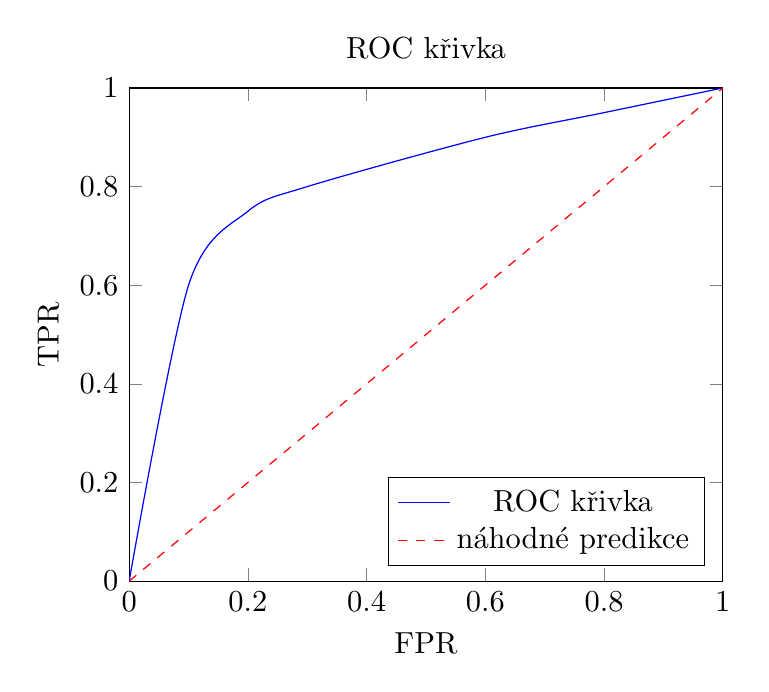
\begin{tikzpicture}[scale=1.1]
        \begin{axis}[
                xlabel={FPR},
                ylabel={TPR},
                title={ROC křivka},
                xmin=0, xmax=1,
                ymin=0, ymax=1,
                legend pos=south east,
            ]

            \addplot[smooth, color=blue] coordinates {(0,0) (0.1,0.6) (0.2,0.75) (0.3,0.8) (0.6,0.9) (0.8,0.95) (1,1)};
            \addlegendentry{ROC křivka}

            \addplot[smooth, color=red, dashed] coordinates {(0,0) (1,1)};
            \addlegendentry{náhodné predikce}

        \end{axis}
    \end{tikzpicture}
\end{center}
Pro dobrý model se křivka přimyká k~levé a horní ose (strmě roste).

\paragraph{AUC}

Kvalita modelu, pro kterou máme ROC křivku, vyhodnocujeme plochou pod křivkou AUC (area under the curve). Model s~náhodnými predikcemi má AUC = 0.5, dokonalý model by měl AUC = 1.

\begin{center}
    \small
    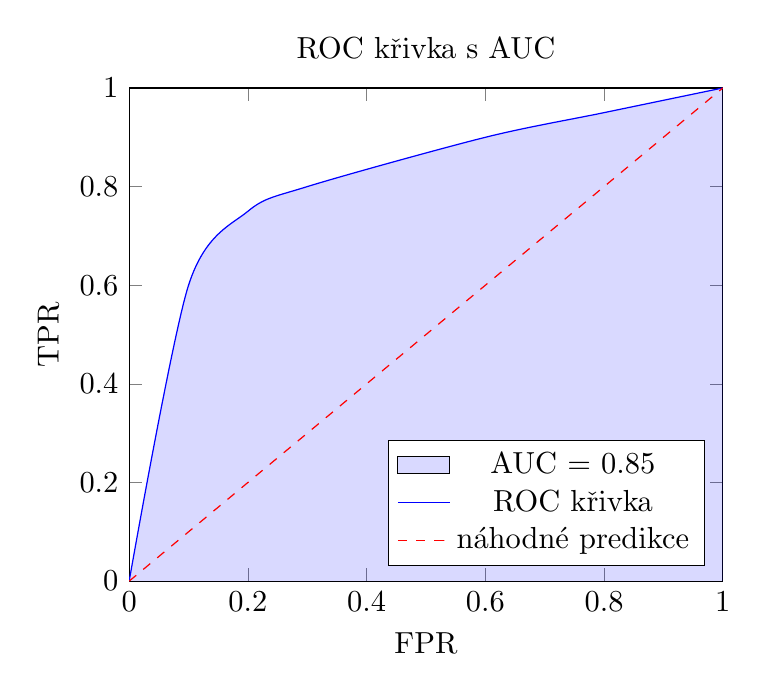
\begin{tikzpicture}[scale=1.1]
        \begin{axis}[
                xlabel={FPR},
                ylabel={TPR},
                title={ROC křivka s~AUC},
                xmin=0, xmax=1,
                ymin=0, ymax=1,
                legend pos=south east,
            ]

            \addplot[fill=blue, fill opacity=0.15, smooth, area legend, draw=none]  coordinates {(0,0) (0.1,0.6) (0.2,0.75) (0.3,0.8) (0.6,0.9) (0.8,0.95) (1,1)} \closedcycle;

            \addplot[smooth, color=blue, line legend] coordinates {(0,0) (0.1,0.6) (0.2,0.75) (0.3,0.8) (0.6,0.9) (0.8,0.95) (1,1)};

            \addplot[smooth, color=red, dashed, line legend] coordinates {(0,0) (1,1)};
            \legend{AUC = 0.85, ROC křivka, náhodné predikce}

        \end{axis}
    \end{tikzpicture}
\end{center}
